\documentclass[xcolor={dvipsnames}]{beamer}

%%% PACKAGES %%%
\usepackage{graphicx}
\usepackage{tabularx}
\usepackage{booktabs}
\usepackage{multirow}
%\usepackage[usenames,dvipsnames]{color}
\usepackage{textpos}
\usepackage{tipa}
\usepackage{hyperref}
%\usepackage{pifont}

%%% RANDOM PACKAGES %%%

%\usepackage{caption}[2008/08/24]
%\usepackage{subcaption}

%\usepackage{enumitem}

%%% FOOTNOTES %%%
\usepackage{perpage}
\MakePerPage{footnote} %restart numbering on each slide

%%% TIKZ %%%
\usepackage{tikz}
\usetikzlibrary{shapes.geometric, arrows}
\tikzstyle{learner} = [rectangle, rounded corners, minimum width=3cm, minimum height=1cm,text centered, draw=black, fill=yellow!30]
\tikzstyle{reference} = [rectangle, rounded corners, minimum width=3cm, minimum height=1cm,text centered, draw=black, fill=green!30]
\tikzstyle{arrow} = [thick,<->,>=stealth]

%%% TODOs %%%
\newcommand{\TODO}[1]{{\color{red}\textbf{[TODO #1]}}}

%%% FONT %%%
\usepackage{tgheros}

%%% BEAMER THEME %%%
\usetheme{default}
\usecolortheme{whale}
\usecolortheme{orchid}
\setbeamertemplate{navigation symbols}{} 
\setbeamertemplate{footline}[frame number]
%\setbeamertemplate{footline}{%
%  \leavevmode%
%  \hbox{%
%    \pgfsetfillopacity{0}\begin{beamercolorbox}[wd=.333333\paperwidth,ht=2.25ex,dp=1ex,center]{author in head/foot}%
%      \usebeamerfont{author in head/foot}\pgfsetfillopacity{1}\insertshortauthor
%    \end{beamercolorbox}%
%    \pgfsetfillopacity{0}\begin{beamercolorbox}[wd=.333333\paperwidth,ht=2.25ex,dp=1ex,center]{title in head/foot}%
%      \usebeamerfont{title in head/foot}\pgfsetfillopacity{1}\insertshorttitle
%    \end{beamercolorbox}%
%    \pgfsetfillopacity{0}\begin{beamercolorbox}[wd=.333333\paperwidth,ht=2.25ex,dp=1ex,right]{date in head/foot}%
%      \usebeamerfont{date in head/foot}\pgfsetfillopacity{1}\insertshortdate{}\hspace*{2em}
%      \insertframenumber{} / \inserttotalframenumber\hspace*{2ex}
%    \end{beamercolorbox}}%
%  \vskip0pt%
%}
\addtobeamertemplate{frametitle}{}{%
\begin{textblock*}{100mm}(.875\textwidth,-.9cm)

\includegraphics[height=.9cm]{uds-logo-text-white.png}
\end{textblock*}}
%\setbeamertemplate{caption}{\insertcaption} %removes "Figure:" etc.
%\setbeamerfont{caption}{size=\scriptsize}
\setbeamertemplate{itemize subitem}[circle]
%\setbeamertemplate{bibliography item}[text]
\setbeamertemplate{bibliography item}[triangle]
\setbeamertemplate{blocks}[rounded][shadow=true]


%%% COLORS %%%
\definecolor{MutedBlue}{RGB}{83,121,170}
\definecolor{UniBlue}{RGB}{0,71,116}
\definecolor{DarkPink}{RGB}{178,56,119}
\definecolor{LightPink}{RGB}{255,224,246}
\definecolor{LightBlue}{RGB}{214,255,255}

%\setbeamercolor{title}{fg=UniBlue}
%\setbeamercolor{frametitle}{fg=UniBlue}
\setbeamercolor{author in head/foot}{fg=UniBlue}
\setbeamercolor{title in head/foot}{fg=UniBlue}
\setbeamercolor{date in head/foot}{fg=UniBlue}
\setbeamercolor{page number in head/foot}{fg=UniBlue}
\setbeamercolor{normal text}{fg=darkgray}
\setbeamercolor{structure}{fg=UniBlue}
\setbeamercolor{itemize item}{fg=UniBlue}
\setbeamercolor{itemize subitem}{fg=UniBlue}
%\setbeamercolor{section in toc}{fg=MutedBlue}
%\setbeamercolor{subsection in toc}{fg=darkgray}
%\setbeamercolor{bibliography entry author}{fg=darkgray}
%\setbeamercolor{bibliography entry title}{fg=darkgray}
%\setbeamercolor{bibliography entry location}{fg=gray!80!black}
%\setbeamercolor{bibliography entry note}{fg=gray!90!black}
%\setbeamercolor{bibliography entry note}{fg=darkgray}
\setbeamercolor{block title}{bg=structure,fg=white}
%\setbeamercolor{block body}{bg={palette secondary}}


%%% BIBLIOGRAPHY %%%
\usepackage[%
	backend=bibtex,
	citestyle=authoryear,
	maxcitenames=2,
	maxbibnames=99,
	firstinits=true,
	url=false,
	doi=false,
	isbn=false, 
	%sorting=none,
	]{biblatex}
\addbibresource{../library.bib}
% to cite on the same slide use \footfullcite{jones00}
\renewcommand{\footnotesize}{\scriptsize}

%% TITLE PAGE INFO %%
\author[A. Vakil]{Anjana Sofia Vakil
%\\\texttt{[anjanav,apalmer]@coli.uni-saarland.de}
} 
\institute{
\includegraphics[height=4.5em]{uds-logo-text.png}\\Department of Computational Linguistics and Phonetics\\University of Saarland, Saarbr{\"u}cken, Germany}
\title{Automatic diagnosis and feedback for lexical~stress errors in non-native speech:\\
Towards a CAPT system for\\French learners of German}
%\subtitle{Investigating the impact of source language choice} 
\date[16.4.15]{Master's Thesis Colloquium\\16 April 2015}

%% DOCUMENT %%
\begin{document}
{
\setbeamertemplate{footline}{} 
\begin{frame}
  \titlepage
\end{frame}
}
\addtocounter{framenumber}{-1}





\begin{frame}{Lexical stress}
Some syllable(s) in a word more accentuated/prominent\footfullcite{Cutler2005}

\begin{center}
\begin{tabular}{ccc}
um$\cdot$FAHR$\cdot$en & vs. & UM$\cdot$fahr$\cdot$en \\
\textit{to run over} & & \textit{to drive around}\\
\end{tabular}
\end{center}

%\vspace{-1em}

\addtocounter{footnote}{-1}
\begin{itemize}
\item{German: variable stress placement, contrastive stress\footnotemark
%\footfullcite{Cutler2005}
}
\item{French: no word-level stress, final syllable lengthening\footfullcite{Michaux2013}}
\end{itemize}

\vfill

Goal: Computer-Assisted Pronunciation Training (CAPT) for lexical stress errors for French learners of German


\end{frame}

\begin{frame}
\frametitle{Outline}
\tableofcontents%[pausesections]
\end{frame}




\section{Motivation}
\begin{frame}{Motivation \TODO{move before outline?}}
		\begin{figure}
			\centering
			\caption{Criteria for selecting errors to target in a CAPT system.}
			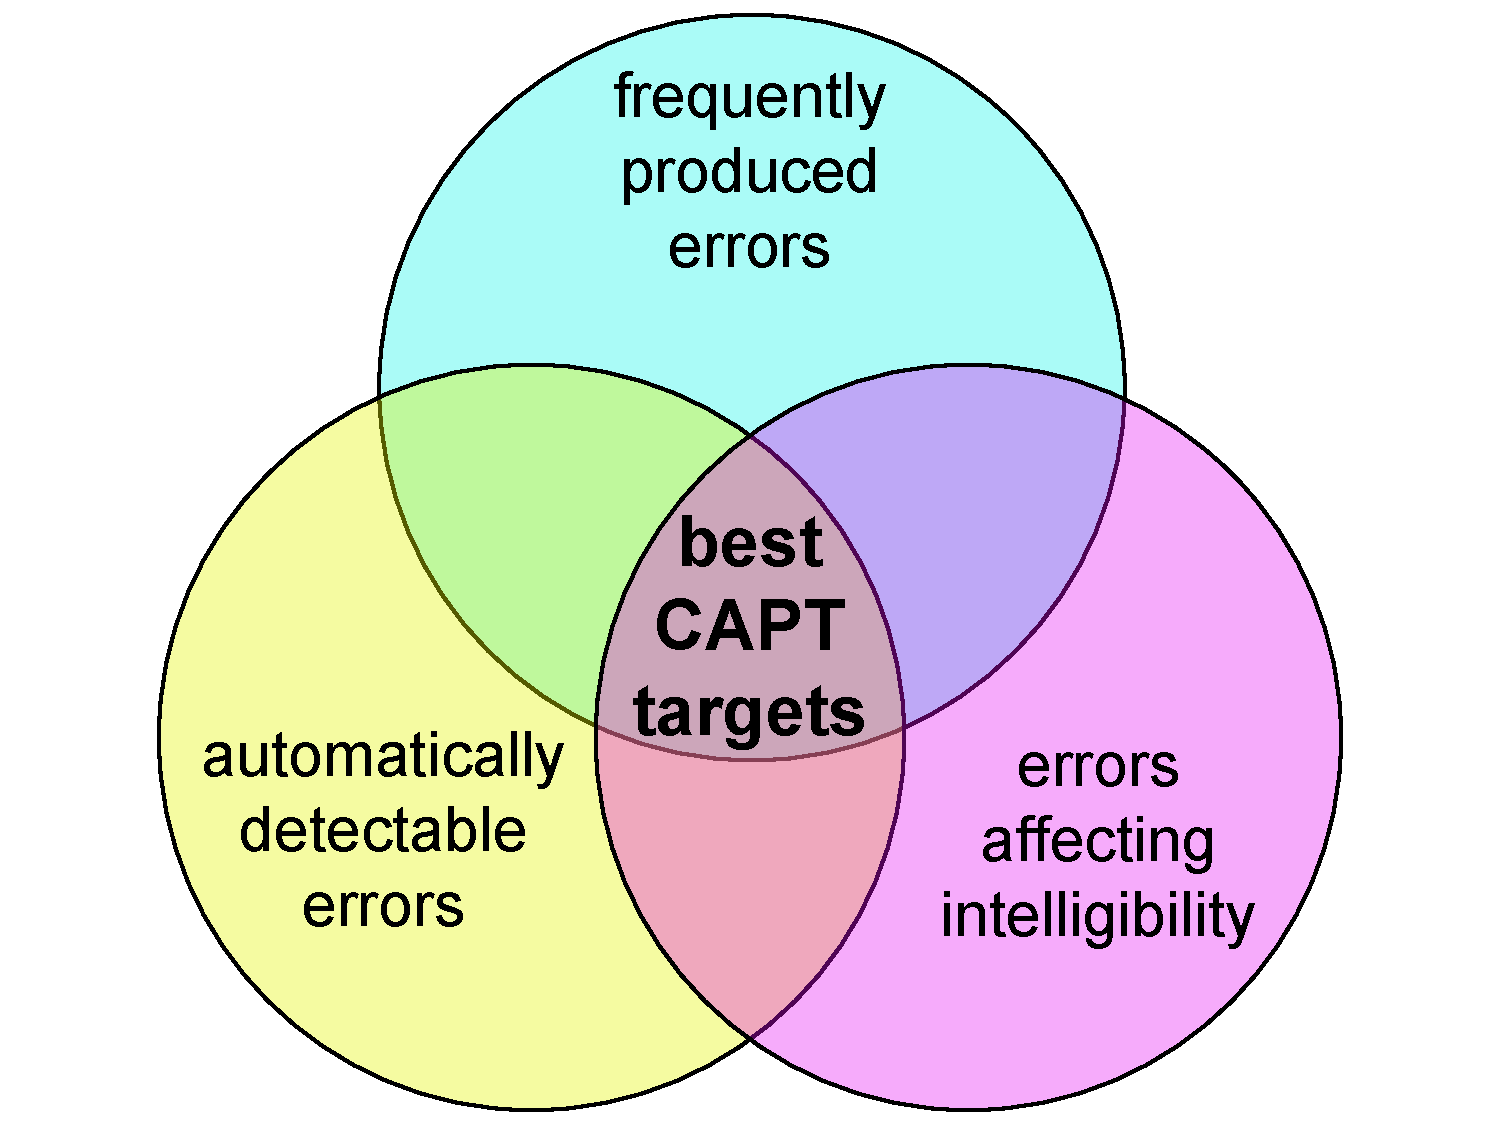
\includegraphics[width=.8\textwidth]{../img/error-venn}
			\label{fig:errors}
		\end{figure}
\end{frame}

\begin{frame}{Motivation \TODO{remove?}}
Lexical stress errors seem to be: 
\begin{itemize}
\item Frequently produced by French learners of variable-stress languages\footfullcite{Bonneau2011}$^{,}$\footfullcite{Michaux2012}
\item More important for intelligibility in L2 German than other types of errors\footfullcite{Hirschfeld1994}
\item Possible to identify automatically by comparison$^1$ or classification\footfullcite{Kim2011}
\end{itemize}

\end{frame}

%\begin{frame}{Motivation}
%Frequently produced:
%\begin{itemize}
%\item French speakers perceptually ``deaf'' to Spanish stress\footfullcite{Dupoux1997}
%\item French learners make stress errors in Dutch\footfullcite{Michaux2012} and English\footfullcite{Bonneau2011}
%%\item French learners of Dutch (incorrectly) stress final syllables\footfullcite{Michaux2012}
%%\item French beginners frequently misplace English stress\footfullcite{Bonneau2011}
%\end{itemize}
%
%Affecting intelligibility:
%\begin{itemize}
%\item Prosodic errors impede intelligibility more than segmental errors
%\item Lexical stress errors have particularly strong impact on L2 German intelligibility\footfullcite{Hirschfeld1994}
%\end{itemize}
%
%
%Automatically detectable:
%
%\end{frame}

\section{Lexical stress errors by French learners of German}
		\begin{frame}{Lexical stress errors in learner speech}
		\begin{itemize}
		\item{How reliably can human annotators identify errors in learner utterances?}
		\vspace{1em}
		\item{How frequently are  errors actually produced by French learners of German?}
		\end{itemize}
		

		\end{frame}
		
	\subsection{Annotation of a learner speech corpus}
		\begin{frame}{Error annotation}
		Data: IFCASL corpus of French-German L1/L2 speech\footfullcite{Fauth2014}
		\begin{itemize}
			\item{German utterances by French and German speakers
				\begin{itemize}
				\item Adults ($>$18) and children (15-16)
				\item Levels A2, B1, B2, C1 (children all A2/B1)
				\end{itemize}
			}
			\item{Word- and phone-level segmentations\\(syllable level added automatically)}
			\item{Selected 12 word types (bisyllabic, initial stress)}
			%TODO word type list on handout?
			%\item{No lexical stress error annotation}

		\end{itemize}
		
		\vfill
		Dataset for annotation:\\
		\hspace*{20pt} 668 word utterances by 55-56 L1 French speakers
		\end{frame}
		
		\begin{frame}{Error annotation}		
		15 Annotators, varying by: \TODO{make this a matrix?}
		\begin{itemize}
			\item{Native language (L1): 
				\begin{itemize}
				\item 12 German 
				\item 2 English (US)
				\item 1 Hebrew
				\end{itemize}
				}
			\item{Phonetics/phonology expertise: 
				\begin{itemize}
				\item 2 Experts
				\item 10 Intermediates
				\item 3 Novices
				\end{itemize}
			}
%			\item{Annotated 3 word types in one $\sim$15 min. session \\(1 annotator did 6 word types in 2 sessions)
%			}
		\end{itemize}
		
		\vfill
		\TODO{5 labels, remove the below}
		
		Each annotated 3 word types in one $\sim$15 min. session \\(1 annotator did 6 word types in 2 sessions)
		
%		\vfill 
%		
%		Task: label each word utterance as:
%						
%			\vspace{.5em}
%			{\small
%
%			\begin{tabular}{rll}
%				& $[$correct$]$ & stress on initial syllable \\
%				& $[$incorrect$]$ & stress on final syllable \\
%				& $[$none$]$ & no clear stress \\
%				& $[$bad\_nsylls$]$ & incorrect number of syllables \\
%				& $[$bad\_audio$]$ & technical problems \\
%			\end{tabular}
%			}
		\end{frame}
		
		\begin{frame}{Error annotation: Method \TODO{remove}}
		\begin{figure}
			\centering
			\caption{Praat annotation tool}
			\includegraphics<1>[height=.75\textheight]{../img/screenshots/AnnotationTool}
			\includegraphics<2>[height=.75\textheight]{AnnotationTool-withLabels}
			%\caption[A screenshot of the graphical annotation tool scripted in Praat.]{A screenshot of the graphical annotation tool scripted in Praat. Green buttons allow the annotator to listen to  the word and sentence utterances. Gray buttons allow the annotator to record their judgment of stress accuracy; from top to bottom, the buttons correspond to the labels [correct], [incorrect], [none], [bad\_nsylls], and [bad\_audio].}
			\label{fig:annotationtool}
		\end{figure}
		\end{frame}
		
%		\begin{frame}{Error annotation}
%		\begin{itemize}
%			\item{
%			12 word types extracted from IFCASL sentences
%			\begin{itemize}
%				\item{bisyllabic (simple syllable comparison)}
%				\item{initial stress (difficult for French speakers)}
%			\end{itemize}
%			}
%			\item{668 word utterances in total (55-56 speakers)}
%			\item{
%			Multiple annotators label each word utterance as: 
%						\vspace{.25em}
%			{\small
%
%			\begin{tabular}{rll}
%				& $[$correct$]$ & stress on initial syllable \\
%				& $[$incorrect$]$ & stress on final syllable \\
%				& $[$none$]$ & no clear stress \\
%				& $[$bad\_nsylls$]$ & incorrect number of syllables \\
%				& $[$bad\_audio$]$ & technical problems \\
%			\end{tabular}
%			}
%%			\begin{tabular}{rll}
%%				{\footnotesize\color{UniBlue} $\bullet$} & $[$correct$]$ & stress on initial syllable \\
%%				$\bullet$ & $[$incorrect$]$ & stress on final syllable \\
%%				$\bullet$ & $[$none$]$ & no clear stress \\
%%				$\bullet$ & $[$bad\_nsylls$]$ & incorrect number of syllables \\
%%				$\bullet$ & $[$bad\_audio$]$ & technical problems \\
%%			\end{tabular}
%%%			\begin{itemize}
%%%				\item{[correct]: stress on initial syllable}
%%%				\item{[incorrect]: stress on final syllable}
%%%				\item{[none]: no clear stress}
%%%				\item{[bad\_nsylls]: incorrect number of syllables}
%%%				\item{[bad\_audio]: technical problems}
%%%			\end{itemize}
%			}
%		\end{itemize}
%		
%		\end{frame}
%		
		
	\subsection{Inter-annotator agreement}
		\begin{frame}{Inter-annotator agreement}
		\textit{How reliably can human annotators identify errors in learner utterances?}
		\vspace{1em}
		\begin{itemize}
		\item Agreement calculated for each overlapping pair
		\item Quantified by:
			\begin{itemize}
			\item Percentage agreement: N agreed/N both annotated
			\item Cohen's Kappa\footfullcite{Cohen1960} ($\kappa$): accounts for chance agreement
			\end{itemize}
		\item \TODO{\textit{remove?}} Overall agreement represented by mean, minimum, median, and maximum of all pairwise values
		\end{itemize}
		
%		\begin{table}%[b]
%			\centering
%			\caption{Overall pairwise agreement between annotators}
%			\begin{tabular}{lrr}
%			\toprule
%				&	\% Agreement	&	Cohen's $\kappa$	\\
%			\midrule
%Mean		&	54.92\%	&	0.23	\\
%Maximum	&	83.93\%	&	0.61	\\
%Median		&	55.36\%	&	0.26	\\
%Minimum	&	23.21\%	&	-0.01	\\
%			\bottomrule
%			\end{tabular}			
%			\label{tab:agreement:overall}
%		\end{table}
		\end{frame}
		
		\begin{frame}{Inter-annotator agreement}
		\begin{table}%[b]
			\centering
			\caption{Overall pairwise agreement between annotators}
			\begin{tabular}{lrr}
			\toprule
				&	\% Agreement	&	Cohen's $\kappa$	\\
			\midrule
Mean		&	54.92\%	&	0.23	\\
Maximum	&	83.93\%	&	0.61	\\
Median		&	55.36\%	&	0.26	\\
Minimum	&	23.21\%	&	-0.01	\\
			\bottomrule
			\end{tabular}			
			\label{tab:agreement:overall}
		\end{table}
		
		\begin{itemize}
		\item{Rather low agreement (``fair''\footfullcite{Landis1977} mean $\kappa$)}
		\item{Large variability between annotators}
		\item{Not explained by L1/expertise groups}
		\end{itemize}
		\end{frame}	
		
		\begin{frame}{Choosing gold-standard labels}
		\TODO{Find more graphical way to portray this? Remove?}
		
		Need a single label for each utterance to analyze error frequency \& evaluate automatic diagnosis		
		\begin{itemize}
		\item 268 utterances: no disagreement 
		\item 265 utterances: majority vote
		\item remaining 135 utterances decided by rules, e.g.: 
			\begin{itemize}
			\item favor Expert judgments
			\item favor certainty ([correct],[incorrect]) over [none]
			\item be generous to learners if [correct] vs. [incorrect]
			\end{itemize}
		\end{itemize}
		\end{frame}
		
	\subsection{Frequency \& distribution of errors}
		\begin{frame}{Error distribution}
		\textit{How frequently are  errors actually produced by French learners of German?}
		
		
		
		%TODO put on handout?
%			\begin{table}
%			\centering
%			\caption{Overall frequency of lexical stress errors in the annotated data}
%			\begin{tabular}{lrr}
%			\toprule
%			Label & Tokens & \% of corpus \\
%			\midrule
%			correct	& 426	& 63.77\% \\
%			incorrect &	198	& 29.64\% \\
%			none	 &35 &	5.24\% \\
%			bad\_nsylls	& 8	& 1.20\% \\
%			bad\_audio	& 1	& 0.15\%\\
%			\midrule
%			%\addlinespace
%			Total & 668 & 100\%\\
%			\bottomrule
%			\end{tabular}
%			\label{tab:results:overall}
%		\end{table}
		
		
		\begin{figure}
			\centering
			%\caption{Overall distribution of lexical stress errors in annotated data}
			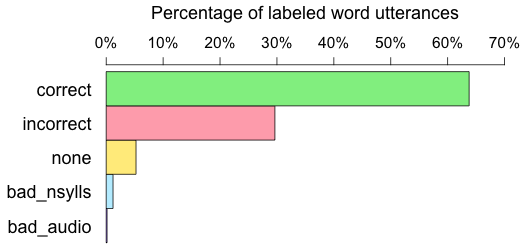
\includegraphics[width=.8\textwidth]{overallJudgments-axisTop-noLabels}

			\label{fig:results:overallbars}
		\end{figure}
		
		\begin{itemize}
		\item Large variability across word types %TODO put by-word table on handout? 
		\item Beginners made more errors (vs. advanced)
		\item Children made more errors (vs. adult beginners)
		\end{itemize}
		\end{frame}
		
%		\begin{frame}{Error distribution by level/age}
%		\TODO{If including this, need to say more about the IFCASL speakers earlier on (or somewhere)}
%		\end{frame}

\section{Diagnosis}
	\subsection{Word prosody analysis}
		\begin{frame}{Word prosody analysis}
		Requires word, syllable, and phone segmentations
			\begin{itemize}
			\item Automatically produced via forced alignment\footfullcite{Mesbahi2011}
			\item This work uses existing IFCASL segmentations
			\item Syllable segmentations derived from words \& phones
			\end{itemize}
			
			\TODO{segmentation screenshot}
		\end{frame}
		
		\begin{frame}{Word prosody analysis: Duration}
		Duration (DUR)
			\begin{itemize}
			\item Perceptual correlate: length/timing
			\item Best indicator of German stress\footfullcite{Dogil1999}
			\item Simple to extract from segmentations
			\item Features: Relative syllable \& nucleus (vowel) lengths
			\end{itemize}
				
		\end{frame}		
		
		\begin{frame}{Word prosody analysis: F0}
		 Fundamental frequency (F0)
			\begin{itemize}
			\item Perceptual correlate: pitch
			\item 2nd best indicator of stress after duration\footfullcite{Dogil1999}
			\item Pitch contours computed using JSnoori\footnote{jsnoori.loria.fr}$^{,}$\footfullcite{DiMartino1999}
			\item Features: relative syllable \& nucleus:
				\begin{itemize}
				\item Mean F0 (in voiced segments)
				\item Maximum F0
				\item Minimum F0 
				\item F0 range (max$-$min)
				\end{itemize}
			\end{itemize}
		\end {frame}
			
		\begin{frame}{Word prosody analysis: Intensity}
		Intensity (INT)
			\begin{itemize}
			\item Perceptual correlate: loudness
			\item Worse predictor than DUR or F0, but still may have effect on stress perception\footfullcite{Cutler2005}
			%\addtocounter{footnote}[-2]
			\item Energy contours computed using Jsnoori
			\item Features: relative syllable \& nucleus:
				\begin{itemize}
				\item Mean energy (over 60dB ``silence threshold'')
				\item Maximum energy
				\end{itemize}
			\end{itemize}
		\end{frame}
		
		
	\begin{frame}{Diagnosis methods}
	\TODO{Slide previewing comparison vs. classification?}
	\end{frame} 
	
	\subsection{Diagnosis by comparison}
%		\begin{frame}{Diagnosis by comparison}
%%		\begin{itemize}
%%		\item 
%%		Common approach in CAPT\footfullcite{Eskenazi2009}
%%		\item Requires L1 reference utterance(s) of same word
%%		\end{itemize}
%		
%		
%		
%			\begin{tikzpicture}
%				\node (stud) [learner] {Learner (L2) utterance};
%				\node (single) [left of=stud, xshift=-2cm] {Single};
%				\node (ref) [reference, right of=stud, xshift=4cm] {Reference (L1) utterance};
%				\draw [arrow] (stud) -- (ref);
%			\end{tikzpicture}
%		
%		\vfill	
%		 
%			\begin{tikzpicture}
%				\node (stud) [learner] {Learner utterance};
%				\node (multi) [left of=stud, xshift=-2cm] {Multiple};
%
%				\node (ref2) [reference, right of=stud, xshift=4cm] {Reference 2};
%				\node (ref1) [reference, above of=ref2, yshift=.3cm] {Reference 1};
%				\node (etc) [below of=ref2] {$\vdots$};
%				\node (refn) [reference, below of=etc] {Reference $n$};
%				\draw [arrow] (stud.north east) -- (ref1.west);
%				\draw [arrow] (stud.east) -- (ref2.west);
%				\draw [arrow] (stud.south east) -- (refn.west);
%			\end{tikzpicture}
%		
%		
%		\end{frame}
		
		\begin{frame}{Diagnosis by comparison}
		Comparison to a single reference utterance
		
		%\vfill
		
		\begin{center}
			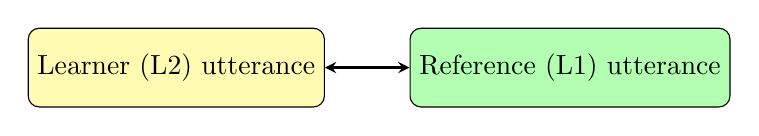
\begin{tikzpicture}
				\node (stud) [learner] {Learner (L2) utterance};
				%\node (single) [left of=stud, xshift=-2cm] {Single};
				\node (ref) [reference, right of=stud, xshift=4cm] {Reference (L1) utterance};
				\draw [arrow] (stud) -- (ref);
			\end{tikzpicture}		
		\end{center}
		
		%\vspace{1em} 
		
		\begin{itemize}
		\item Simplest approach, common in CAPT%\footfullcite{Eskenazi2009}
		\item JSnoori (and predecessors) use this method\footfullcite{Bonneau2011}
			\begin{itemize}
			\item Assigns 3 scores (DUR, F0, INT)
				\begin{itemize}
				\item Same syllable stressed?
				\item Difference between stressed/unstressed syllables similar enough?
				%\item Each score based on stress placement \& difference between stressed-unstressed syllables
				\end{itemize}
			\item Overall score = weighted average of 3 scores
			\end{itemize}
		\item Problem: extremely utterance-dependent!
		\end{itemize}
		\end{frame}
		
		\begin{frame}{Diagnosis by comparison}
		Comparison to multiple reference utterances
		
		\begin{center}		
		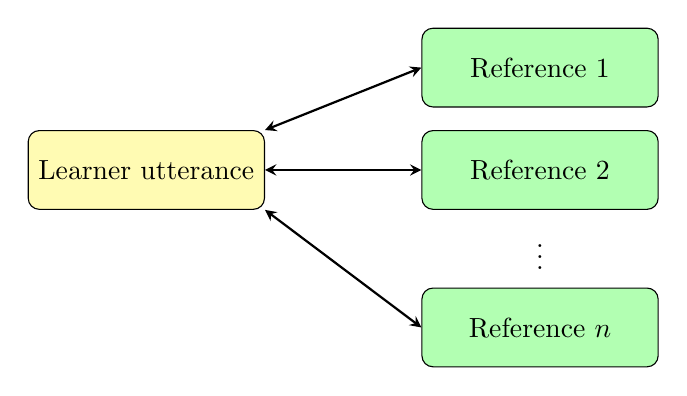
\begin{tikzpicture}
			\node (stud) [learner] {Learner utterance};
			%\node (multi) [left of=stud, xshift=-2cm] {Multiple};

				\node (ref2) [reference, right of=stud, xshift=4cm] {Reference 2};
			\node (ref1) [reference, above of=ref2, yshift=.3cm] {Reference 1};
			\node (etc) [below of=ref2] {$\vdots$};
			\node (refn) [reference, below of=etc] {Reference $n$};
			\draw [arrow] (stud.north east) -- (ref1.west);
			\draw [arrow] (stud.east) -- (ref2.west);
			\draw [arrow] (stud.south east) -- (refn.west);
		\end{tikzpicture}
		\end{center}
			
		\begin{itemize}
		\item Less common in CAPT systems
		\item Less utterance-dependent than single comparison
		\item Overall score = average of one-on-one scores
		\end{itemize}
		\end{frame}		
		
		\begin{frame}{Diagnosis by comparison}
		Options for selecting reference speaker(s)
		\begin{itemize}
		\item Manually 
			\begin{itemize}
			\item Learner's choice
			\item Teacher/researcher's choice
			\end{itemize}
		\item Automatically 
			\begin{itemize}
			\item May be more effective to choose reference speaker most closely resembling the learner\footfullcite{Probst2002}
			\item Selected by comparing speakers' F0 mean and range (using all available recordings)
			\end{itemize}
		\end{itemize}
		
		\end{frame}
		
		
		
	\subsection{Diagnosis by classification}
		\begin{frame}{Diagnosis by classification}
		\begin{itemize}
		\item More abstract representation of L1 pronunciation
		\item Not yet explored for German CAPT
		%\item One of main contributions of this thesis
		\end{itemize}
		\vfill
		Research questions:
		\begin{itemize}
		\item \textit{How well can lexical stress errors be classified?}
		\item \textit{How does that compare with human agreement?}
		\item \textit{Which features are most useful for classification?}
		\end{itemize}	
		\end{frame}	
		
		\begin{frame}{Diagnosis by classification}
		Experiments:
		\begin{itemize}
		\item Trained CART classifiers using WEKA toolkit\footnote{www.cs.waikato.ac.nz/ml/weka}
		\item Used annotated L2 dataset for training/test data
		\item Used L1 utterances of the same words as training data \\(all automatically labeled [correct])
		\end{itemize}
		
		\vfill
		
		Evaluated in terms of:
		\begin{itemize}
		\item Agreement (\%, $\kappa$) with gold-standard labels
		\item Precision, Recall, F$_1$ and F$_2$ for [correct] class \TODO{explain and/or put on handout}
		\end{itemize}
		\end{frame}

		\begin{frame}{Diagnosis by classification}
		\textit{Which features are most useful for classification?}
		\vfill
		\begin{tabularx}{\textwidth}{lX}
			%\begin{tabular}{ll}
			\toprule
			Feature set & Description \\
			\midrule
			DUR & Duration features \\
			F0 & Fundamental frequency features \\
			INT & Intensity features \\
			\midrule
			WD %WORD 
				& Uttered word (e.g. \textit{Tatort}) \\
			LV % LEVEL 
				& Speaker's L2 German skill level  (A2$|$B1$|$B2$|$C1)\\
			AG %GENDER 
				& Speaker's age/gender  (Girl$|$Boy$|$Woman$|$Man)\\
%			LV+AG & LEVEL, GENDER \\
%			WD+LV & WORD, LEVEL \\
%			WD+AG & WORD, GENDER \\
%			WD+SPKR & WORD, LEVEL, GENDER \\
			\bottomrule
			\end{tabularx}		
		
%		\begin{itemize}
%		\item Prosodic features
%			\begin{itemize}
%			\item DUR -Duration
%			\item F0 - Fundamental frequency
%			\item INT - Intensity 
%			\end{itemize}
%		\item WD - Word type (e.g. \textit{Flagge})
%		\item Speaker features
%			\begin{itemize}
%			\item LV - German proficiency level (A2$|$B1$|$B2$|$C1)
%			\item AG - Age/gender (Girl$|$Boy$|$Woman$|$Man)
%			\end{itemize}
%		\end{itemize}
		\end{frame}


		\begin{frame}{Diagnosis by classification}
		\begin{figure}
		\includegraphics<1>[width=\textwidth]{results-prosodicfeatures}
		\includegraphics<2>[width=\textwidth]{results-prosodicfeatures-highlight}
		\end{figure}
		
		\vfill
		\pause
		Best performance using only prosodic features: DUR+F0
		\begin{itemize}
		\item \% Accuracy: 69.77\% 
		\item $\kappa$: 0.29
		\end{itemize}
		\end{frame}



\section{Feedback}
	\subsection{Implicit}
		\begin{frame}{Implicit feedback}
		\TODO{}
		\end{frame}
	\subsection{Explicit}
		\begin{frame}{Explicit feedback}
		\TODO{}
		\end{frame}
	\subsection{Self-assessment}
		\begin{frame}{Self-assessment}
		\TODO{}
		\end{frame}

	
\section{The de-stress CAPT tool }
%	\subsection{For students}
%		\begin{frame}{\TODO{}}
%		\TODO{}
%		\end{frame}
%	\subsection{For teachers/researchers}
		\begin{frame}{\TODO{}}
		\begin{itemize}
		\item Create Exercise
		\item Create DM
			\item Create Scorer?
		\item Create FM
		\item Show FB output
		\end{itemize}
		\end{frame}


\end{document}